\documentclass{beamer}

%\usepackage{subfigure}
\usepackage{graphicx}
\usepackage{sidecap}
\usepackage{caption}
\usepackage{subcaption}
\captionsetup{compatibility=false}
\usepackage{appendixnumberbeamer}
\usepackage{amsmath}
% --
\usepackage{multirow}
\usepackage{xcolor}
\usepackage{setspace}
\usepackage{hyperref}
\usepackage{anyfontsize}

\setbeamertemplate{footline}

\newenvironment{itemise} {\begin{itemize} \setlength{\itemsep}{0.2cm}} {\end{itemize}}
\usepackage[labelformat=empty]{caption}
\setbeamertemplate{sections/subsections in toc}[square]

%% COLORS
\definecolor{Gray}{gray}{0.9}
\definecolor{dblue}{rgb}{0.132,0.1,0.27}
\definecolor{mint}{cmyk}{1.0, 0.2, 0.6, 0.05}
\definecolor{ant}{cmyk}{0.5, 0.1, 0.0, 0.45}
\definecolor{lgray}{cmyk}{0.12, 0.0, 0.0, 0.17}
\definecolor{lred}{cmyk}{0.0, 0.9, 0.7, 0.0}


\usepackage{etoolbox}% http://ctan.org/pkg/etoolbox 
\usepackage{booktabs}

\newenvironment{literatur}{%
  \parskip2pt \parindent0pt \raggedright
  \def\lititem{\hangindent=0.5cm \hangafter1}}{%
  \par\ignorespaces}

\newcommand{\tb}[1]{{\color{blue}{\textbf{#1}}}}
\newcommand{\tm}[1]{{\color{mint}{\textbf{#1}}}}
\newcommand{\tr}[1]{{\color{red}{\textbf{#1}}}}
% Ilya: packages

\usepackage{tikz}
\usepackage{lmodern}
\usepackage{enumitem}

% Ilya: my commands

\newenvironment{mytemize}
{\vfill\itemize[nolistsep,itemsep=\fill,label=\color{blue}{$\triangleright$}]}
  {\enditemize}


\newenvironment{mynumerate}
{\vfill\enumerate[nolistsep,itemsep=\fill,label=\arabic*.]}
  {\endenumerate}

\newcommand{\hitem}[1]{
  {\color{blue}{$\triangleright$}} 
  {#1} 
  {\hfill}
}

\setlist[itemize]{label= \color{blue}{$\triangleright$}}
\setlist[enumerate]{label = \arabic*.}

\newcommand{\rarr}{$\Rightarrow$\ }

%------------------------------------------------------------------------------------
% TITLE
%------------------------------------------------------------------------------------
\title[PSME]{Macroeconomics\\ Lecture 9 -- New Keynesian Model II}
\author[I. Eryzhenskiy]{Ilya Eryzhenskiy}
\institute[Paris-1]{PSME Panth\'{e}on-Sorbonne Master in Economics}
\date[PSME macro]{Fall 2022}

%---BEGIN------------------------------------------------------------------------------
\begin{document}
%---BEGIN------------------------------------------------------------------------------
\begin{frame}
\maketitle
\end{frame}
%---FRAME------------------------------------------------------------------------------
%\section{Outline}
\begin{frame}
\frametitle{Outline}
\tableofcontents
\end{frame}
\section{Nominal rigidities}
\begin{frame}
\frametitle{Outline}
\tableofcontents[currentsection]
\end{frame}
\begin{frame}{Nominal rigidities, a.k.a. sticky prices}

\begin{mytemize}
\item How sticky are prices? 
\item Empirical work (Dhyne et al, 2005) $\rightarrow$ average duration of a price spell is \textbf{4-5 quarters} in the EU
\item How to build this in the New Keynesian model?
\item[$\rightarrow$] Common sticky price mechanisms:
\begin{enumerate}
  \item \tb{Calvo pricing: exogenous probability that firm can change price at a given period}
\item \emph{Rotemberg pricing}: firm can change price every period, but s.t. a quadratic 'menu cost'
\item \emph{Taylor contracts}: firm can change price every $T$ periods
\end{enumerate}
\end{mytemize}
We will look at Calvo pricing -- most common and convenient assumption, although most ``unrealistic'' one

\end{frame}
%---FRAME------------------------------------------------------------------------------
\begin{frame}{Calvo pricing}

\begin{mytemize}
\item Every period, each firm may change price with probability $1-\alert{\theta}$
\item[$\Rightarrow$] at a given period, fraction $\alert{\theta}$ of firms keeps price unchanged
\item[$\Rightarrow$] fraction $1-\alert{\theta}$ can set new price
\item average duration of a price $1/(1-\alert{\theta})$ periods 
  \begin{mytemize}
  \item can set $\theta$ to match a target duration, e.g. 5 quarters	
  \end{mytemize}
\end{mytemize}


\end{frame}
%---FRAME------------------------------------------------------------------------------
\begin{frame}{Aggregate price dynamics}
\begin{align}
  (\underbrace{\frac{P_t}{P_{t-1}}}_{1+\pi_t} )^{1-\varepsilon} = \alert{\theta} + (1-\alert{\theta}) ( \frac{P_t^*}{P_{t-1}} )^{1-\varepsilon} \nonumber%, \label{aggprice_level}
\end{align}
with $P^*_t$ the optimal price set in period $t$ by firms that can change price. Firms identical \rarr $P^*_t$ same for all.

\medskip
Log-linearized using Taylor series around steady state with $P_t/P_{t-1}=1$  and $P_t^*/P_{t-1}=1$:
\begin{align}
  \pi_t = (1-\theta) (p^*_t-p_{t-1}) \label{aggprice_log}
\end{align}

\begin{mytemize}
\small
\item How are prices $P^*_t$ chosen? $\rightarrow$ coming up next. We will skip some of the algebra; for full derivation, see notes of Drago Bergholt: 
\vfill
  \url{https://bergholt.weebly.com/uploads/1/1/8/4/11843961/the_basic_new_keynesian_model_-_drago_bergholt.pdf}
\end{mytemize}
\end{frame}
%---FRAME------------------------------------------------------------------------------
\section{Firm problem with Calvo pricing}
\begin{frame}
\frametitle{Outline}
\tableofcontents[currentsection]
\end{frame}
\begin{frame}{Intertemporal profit maximization: discounting}
  Firm chooses price for (uncertain) number of periods \rarr profit maximization involves many periods.
  \vfill 
  How to value future profits? With households' relative utility of future consumption, also known as \tb{stochastic discount factor (SDF)} $Q_{t,t+k}$:
  \vfill
  \begin{mytemize}
  \item 	
  Consider a small nominal payment $\epsilon$ obtained in future period $t+k$. Expected utility in period $t$:
  $$\beta^{t+k} E_t \underbrace{(1-\sigma)C^{-\sigma}_{t+k}}_{\frac{\partial U}{\partial C}} \underbrace{\frac{\epsilon}{P_{t+k}}}_{\text{units of} C_{t+k}}$$
\item Suppose the household pays $Q_{t, t+k}\epsilon $ at $t$ to obtain this future payment, so that $Q_{t, t+k}$ is the price of 1 unit of money received $k$ periods in future. Utility: 
  $$ \beta^{t} (1-\sigma)C^{-\sigma}_{t} \frac{Q_{t, t+k}\epsilon}{P_{t}}$$
  \end{mytemize}
  If $Q_{t,t+k}$ is the right value of future payment, the utilities are equal. The \tb{SDF} is then \tb{$Q_{t, t+k} = \beta^k (C_{t+k}/C_t)^{-\sigma} (P_t/P_{t+k})$}
\end{frame}

\begin{frame}{Firms: Optimal price setting}

\begin{mytemize}
\item Choice of price maximizes stream of expected future profits, discounted with households' SDF:
  $$\max_{P_t^*} E_t \sum_{k = 0}^{\infty} Q_{t, t+k} \Pi^N_{t+k}$$
\item Denote $\Pi^N_{t+k \mid t}$ nominal profit at period $t+k$ of firm that last chose price at $t$
\item For a firm setting price in current period $t$, maximization of profit of the period is as in flex price model: 
$$\Pi^N_{t\mid t} = P^*_t Y_{t\mid t}-TC^N_{t}(Y_{t \mid t})$$
with $Y_{t \mid t} = \left( \frac{P^*_{t}}{P_{t}}\right)^{-\varepsilon} C_{t}$

\item For a firm that hasn't changed price for a while, it is:
$$\Pi^N_{t+k\mid t} = P^*_t Y_{t+k\mid t}-TC^N_{t+k}(Y_{t+k \mid t})$$
with $Y_{t+k \mid t} = \left( \frac{P^*_{t}}{P_{t+k}}\right)^{-\varepsilon} C_{t+k}$
\end{mytemize}
\end{frame}

\begin{frame}{Firms: Optimal price setting}
  Nominal profit $\Pi^N_{t+k}$ depends on $P_t^*$ \alert{only if firm never could change price between $t$ and $t+k$}. Probability is $\theta^k$
	\vfill
Expected nominal profit can be rewritten $$E_t \Pi^N_{t+k} = \theta^k \Pi^N_{t+k\mid t} + (1-\theta)\theta^{k-1} \Pi^N_{t+k\mid t+1} + 
  (1-\theta)^2\theta^{k-2} \Pi^N_{t+k\mid t+2} + \dots$$
  \begin{mytemize}
  \item only first term depends on $P^*_t$ \rarr all other terms ignored in period $t$ maximization
  \end{mytemize}
  \vfill
  Finally, maximization problem can be rewritten:
  \begin{align*}
	\max_{P_t^*} &\sum_{k = 0}^{\infty} \alert{\theta^k} E_t Q_{t, t+k} [P^*_t Y_{t+k\mid t}-TC^N_{t+k}(Y_{t+k \mid t})] \\
\text{s.t.} \ \  &Y_{t+k \mid t} = \left( \frac{P^*_{t}}{P_{t+k}}\right)^{-\varepsilon} C_{t+k}
  \end{align*}
\end{frame}
%---FRAME------------------------------------------------------------------------------
\begin{frame}{Firms: Optimal price setting}


\textbf{Solution} FOC w.r.t. $P^*_t$:
\begin{align}
\sum_{k=0}^{\infty} \theta^k E_t \left[ Q_{t,t+k} Y_{t+k \mid t} (P^*_t - \frac{\varepsilon}{\varepsilon-1} MC^N_{t+k \mid t})\right] = 0 \nonumber
\end{align}
with 
\begin{mytemize}
\small
\item $MC^N_{t+k \mid t} \equiv \frac{d}{d Y}TC^N_{t+k}(Y_{t+k \mid t})$: nominal marginal cost in period $t+k$
\item $\frac{\varepsilon}{\varepsilon-1}$: desired (flexible-price) mark-up over marginal costs 
\end{mytemize}
\vfill
Flexible price solution obtains under $\theta=0$:
\begin{equation*}
  P^*_t = \frac{\varepsilon}{\varepsilon-1} MC^N_{t \mid t} \quad \text{for each}\ t
\end{equation*}
\end{frame}
%---FRAME------------------------------------------------------------------------------
\begin{frame}{Firms: Optimal price setting}

\begin{align*}
  \sum_{k=0}^{\infty} \theta^k E_t Q_{t,t+k} Y_{t+k \mid t} P^*_t =\frac{\varepsilon}{\varepsilon-1} \sum_{k=0}^{\infty} \theta^k E_t  Q_{t,t+k} Y_{t+k \mid t}   MC^N_{t+k \mid t}
\end{align*}
Using $Q_{t, t+k} = \beta^k (C_{t+k}/C_t)^{-\sigma} (P_t/P_{t+k})$ and solving for $P^*_t$:
\begin{align*}
  P^*_t = \frac{\varepsilon}{\varepsilon-1} \frac{E_t \sum_{k=0}^\infty  \theta^k \beta^k C^{1-\sigma}_{t+k} P^{\varepsilon-1}_{t+k} \textcolor{red}{MC^N_{t+k\mid t}}}{E_t \sum_{k=0}^\infty  \theta^k \beta^k C^{1-\sigma}_{t+k} P^{\varepsilon-1}_{t+k}}
\end{align*}
%where $\textcolor{red}{MC_{t+k\mid t}} \equiv MC^N_{t+k\mid t}/P_{t+k}$ is the real marginal cost in period $t+k$ for a firm whose price was last set in period $t$.
\vfill
\textbf{Optimal price is markup times weighted sum of expected real costs}
\end{frame}
%%---FRAME------------------------------------------------------------------------------
\begin{frame}{Firms: Optimal price setting}

  After doing a (long) log-linearization around steady state with $P_t = P_{t-1} = P; \pi=0$:
\begin{align}
p_t^*-p_{t-1}= (1-\beta \theta) \sum_{k=0}^{\infty}(\beta \theta)^k
E_t [\hat{mc}_{t+k \mid t}+(p_{t+k}-p_{t-1})] \label{pstar-pminus1}
 \end{align}
where $\hat{mc}_{t+k \mid t}\equiv mc_{t+k \mid t}-mc$ denotes the \tb{log deviation} of real marginal cost from its steady state value.

Use $mc = \ln(MC) = \ln(MC^N/P) =  \ln \frac{\varepsilon}{\varepsilon-1} \equiv \mu$ to obtain:

\begin{align*}
p_t^* = \mu + (1-\beta \theta) \sum_{k=0}^{\infty}(\beta \theta)^k
 E_t [mc_{t+k \mid t}+p_{t+k}] 
\end{align*}
\end{frame}
%---FRAME------------------------------------------------------------------------------
\section{Equilibrium}
%---FRAME------------------------------------------------------------------------------
\begin{frame}{Outline}
\tableofcontents[currentsection]
\end{frame}
%---FRAME------------------------------------------------------------------------------
%\begin{frame}{Equilibrium - Goods market}
%
%{
%\footnotesize
%\begin{mytemize}
%\small
%\item \tb{Goods market equilibrium}
%\begin{align*}
%Y_t(i)=C_t(i) \text{ for all }i\in[0,1] \text{ and all }t
%\end{align*}
%defining \tb{aggregate output}
%\begin{align*}
%Y_t \equiv \left(\int_0^1 Y_t(i)^{\frac{\varepsilon-1}{\varepsilon}} di\right)^{\frac{\varepsilon}{\varepsilon-1}}
%\end{align*}
%such that, taken together (\emph{aggregate market clearing condition})
%\begin{align*}
%Y_t = C_t
%\end{align*}
%\end{mytemize}
%}
%
%\end{frame}
%---FRAME------------------------------------------------------------------------------
\begin{frame}{Equilibrium -- aggregate (log) output}

  $Y_{t}(i)$ and $L_t(i)$ vary across firms because of sticky prices \rarr aggregate production function not same as firms' production function.
Recall aggregate labor definition: $L_t = \int_0^1 L_t(i) di$;
using the firms' production function:
\begin{align*}
L_t =& \int_0^1 \left( \frac{Y_t(i)}{A_t}\right)^{\frac{1}{1-\alpha}}di = \left( \frac{Y_t}{A_t}\right)^{\frac{1}{1-\alpha}} \int_0^1 \left( \frac{P_t(i)}{P_t}\right)^{-\frac{\varepsilon}{1-\alpha}} di
\end{align*}
In logs:
\begin{align*}
  (1-\alpha) l_t = y_t -a_t +\mathcal{D}_t \\
  \mathcal{D}_t \equiv (1-\alpha) log \int_0^1 \left( \frac{P_t(i)}{P_t} \right)^{\frac{\varepsilon}{1-\alpha}}
\end{align*}
where $\mathcal D_t$ is a measure of price dispersion. In a first-order approximation around s.s. with $\pi=0$, it is null \rarr simple \textit{approximate} aggregate production function:
\tr{$y_t = a_t + (1-\alpha) l_t$}

\end{frame}
%---FRAME------------------------------------------------------------------------------
\subsection{New Keynesian Phillips Curve}
\begin{frame}{New Keynesian Phillips Curve}
  We need some more algebra (again, presented more fully in Bergholt notes) to obtain a micro-founded version of the \tb{AS relationship} linking inflation and the output gap.
  \vfill 
  Surprisingly, the micro-founded version has been labelled the \tb{New Keynesian Phillips Curve}, although unemployment is out of the picture. 
  \vfill 
  This equation ends up being the only (but crucial) difference between the flexible price and sticky price versions of the model.
\end{frame}
%---FRAME------------------------------------------------------------------------------
\begin{frame}{Inflation and average marginal cost}

  Aggregate price dynamics (7) and optimal price setting of firms \eqref{pstar-pminus1} allow to relate inflation to average marginal costs in the economy. First, $mc_{t+k\mid t}$ is expressed with respect to economy's average marginal costs: 
  \begin{align*}
	mc_{t+k\mid t} = mc_{t+k} + \frac{\varepsilon\alpha}{1-\alpha} (p^*_t - p_{t+k})
  \end{align*}
  After substitution in \eqref{pstar-pminus1} and re-arranging, we get 
  $$p^*_t-p_{t-1} = E_t \sum_{k=0}^\infty \theta^k \beta^k \left((1-\theta \beta)\frac{1-\alpha}{1-\alpha+\alpha \varepsilon} \hat{mc}_{t+k} + \pi_{t+k}\right) $$
  which can be written recursively:
\begin{align*}
p^*_t-p_{t-1} = \beta \theta E_t \left[ p_{t+1}^* -p_t\right]+ (1-\beta \theta) \theta \hat{mc}_t + \pi_t 
\end{align*}
combine with $\pi_t = (1-\theta)(p_t^* - p_{t-1})$ to get:
\begin{align}
  \pi_t &= \beta E_t [\pi_{t+1}]+ \lambda \hat{mc}_t  \label{pi_mc}\\
\text{with } \lambda &\equiv \frac{(1-\theta)(1-\beta \theta)}{\theta}\frac{1-\alpha}{1-\alpha+\alpha \varepsilon} \nonumber
\end{align}
\end{frame}
%---FRAME------------------------------------------------------------------------------
\begin{frame}{Marginal cost and output gap}

  As seen in flex. price model, $mc^N_t = w^N_t + \left(\frac{1}{\alpha-1}\right)a_t + \left(\frac{\alpha}{1-\alpha}\right)y_t$. To get an expression for real log marginal costs $mc_t (= mc^N_t - p_t)$, use households'  consumption-labor optimality $w^N_t - p_t = \sigma y_t + \eta l_t$ and approximate aggregate production $y_t = a_t + (1-\alpha)l_t$ to get:
  $$mc_t =  \left( \sigma + \frac{\eta+\alpha}{1-\alpha}\right) \textcolor{red}{y_t} - \frac{1+\eta}{1-\alpha}a_t - log(1-\alpha)$$

  The steady state log real marginal cost is $-\mu$ but can also be related to \tb{output under flexible prices} or \tb{natural output} $y^n_t$: 
  $$mc = \left( \sigma + \frac{\eta+\alpha}{1-\alpha}\right) \textcolor{blue}{y^n_t} - \frac{1+\eta}{1-\alpha}a_t - log(1-\alpha)$$
  Finally, log deviation of real marginal cost $\hat mc_t \equiv mc_t - mc$ is related to \tb{log output gap} $\tilde y_t \equiv y_t - y^n_t$: 

  \begin{equation}
\hat{mc_t} = \left( \sigma + \frac{\eta+\alpha}{1-\alpha} \right)(y_t-y^n_t) 
	\label{mc_y}
  \end{equation}
\textbf{And we can obtain the New Keynesian Phillips Curve} 
\includegraphics[width=0.8cm]{FIGURES/party_popper.png}
\end{frame}
%---FRAME------------------------------------------------------------------------------
{
\usebackgroundtemplate%
{%
  %\begin{figure}[b!]
  \begin{tikzpicture}
	\draw node[opacity=0] at (15,6) {
\includegraphics[width=0.3\paperwidth]{baby_logo.png}};%
    \draw node[opacity=0.3] at (14.5,-0.4) {
\includegraphics[width=0.3\paperwidth]{FIGURES/finish_flag.png}};%
    %\draw node[opacity=0.8] at (15.3,6) {\includegraphics[width=0.23\paperwidth]{../PSE_logo.png}};%
	\draw node[opacity=0] at (10.3,-1.4) {
\includegraphics[width=0.37\paperwidth]{baby_logo.png}};%
	\draw node[opacity=0] at (6,-1.4) {
\includegraphics[width=0.3\paperwidth]{baby_logo.png}};%
  \end{tikzpicture}
  %\end{figure}
}

%\begin{frame}{Average real marginal costs}
%
%{
%\small
%%[colback=blue!5!white,colframe=blue!75!black,title=Definition]
%%\begin{tcolorbox}
%\tb{Definition:} 
%The natural level of output $y_t^n$ is the equilibrium level of output under flexible prices.
%%\end{tcolorbox}
%
%\begin{mytemize}
%\item Marginal costs in the \emph{flexible prices economy} are constant ($mc=-\mu$) thus the average real marginal costs amount to
%\end{mytemize}
%\begin{align}
%mc = \left( \sigma + \frac{\eta+\alpha}{1-\alpha}\right) \textcolor{blue}{y^n_t} - \frac{1+\eta}{1-\alpha} \textcolor{blue}{a_t} - log(1-\alpha) \tag{18}
%\end{align}
%which implies \emph{(after solving for $y^n_t$)}
%\begin{align}
%y^n_t &= \psi^n_{ya}\textcolor{blue}{a_t} + \vartheta^n_y \tag{19} \\
%\text{with } \psi^n_{ya} &\equiv \frac{1+\eta}{\sigma(1-\alpha)+\eta+\alpha} \nonumber \\
%\text{and } \vartheta^n_t &\equiv  -\frac{(1-\alpha)(\mu-log(1-\alpha))}{\sigma(1-\alpha)+\eta+\alpha} \alert{>0} \nonumber
%\end{align}
%
%}
%\end{frame}
%---FRAME------------------------------------------------------------------------------
\begin{frame}{The New Keynesian Phillips Curve}


  Equation \eqref{mc_y} for marginal cost \& output gap and equation \eqref{pi_mc} for inflation \& marginal cost result in the \tb{New Keynesian Phillips Curve} (NKPC):
\begin{equation}
  \pi_t = \beta Et [\pi_{t+1}]+ \kappa \tilde{y}_t \label{nkpc}
\end{equation}
where $\kappa \equiv \frac{(1-\theta)(1-\beta \theta)}{\theta}\frac{1-\alpha}{1-\alpha+\alpha \varepsilon}
\left(\sigma + \frac{\eta+\alpha}{1-\alpha}\right)$ 
\vfill
Note that $\kappa$ depends negatively on both $\theta$ and $\beta$, which get smaller if period length gets larger \rarr relationship gets steeper as horizon gets longer, as with the old \tb{AS} curve
\end{frame}
}
%---FRAME------------------------------------------------------------------------------
%---FRAME------------------------------------------------------------------------------
\subsection{Dynamic IS curve}
\begin{frame}
\frametitle{Outline}
\tableofcontents[currentsubsection]
\end{frame}
%---FRAME------------------------------------------------------------------------------
\begin{frame}{Dynamic IS curve}

From the Euler equation and goods market equilibrium
$$ y_t = E_t[y_{t+1}]- \frac{1}{\sigma}(\underbrace{i_t-E_t[\pi_{t+1}]}_{r_t}-\rho) $$
while in the flexible price model:
$$ y^n_t = E_t[y_{t+1}]- \frac{1}{\sigma}(r^n_t-\rho) $$
(recall that the \tb{natural real interest rate} $r^n_t$ is entirely driven by fundamentals -- parameters and  productivity) \\
Take a difference \rarr \tb{dynamic IS equation} in terms of the output gap $\tilde y_t$
\begin{align}
  \tilde{y}_t = -\frac{1}{\sigma}(i_t-E_t[\pi_{t+1}]-r^n_t)+E_t[\tilde{y}_{t+1}] \label{is}
\end{align}

\end{frame}
%---FRAME------------------------------------------------------------------------------
\begin{frame}{Dynamic IS curve}

  Note that the dynamic IS is another recursive equation. Iterate forward:

\begin{align*}
  \tilde{y}_t &= - \frac{1}{\sigma} \sum_{k=0}^{\infty} (r_{t+k}-r^n_{t+k}) +\underbrace{\lim_{T\rightarrow \infty} E_t [\tilde{y}_{t+T}]}_{=0}
\end{align*}

\underline{Interpretation:} the output gap is proportional to the sum of current and anticipated deviations between the real interest rate and its natural counterpart.

\end{frame}
%---FRAME------------------------------------------------------------------------------
%\begin{frame}{The natural rate hypothesis}
%
%{
%\small
%\tb{M. Friedman (1968)}
%\begin{enumerate}
%\item There is a natural rate (of unemployment, output) independent of monetary policy (determined by structural characteristics of the labor and commodity markets, including market imperfections.)
%\item Monetary policy can not sustain unemployment (output) below (above) the natural rate without leading to higher and higher inflation (\tb{accelerationist hypothesis})
%\end{enumerate}
%
%\tb{O. Blanchard (JEP 2018)}
%
%\emph{While the natural rate hypothesis was controversial at the time, it quickly became widely accepted, and has been the dominant paradigm in macroeconomics ever since. It is embodied in the thinking and the models used by central banks, and it is the basis of the inflation-targeting framework used by most central banks today.} \emph{[Discussion later ...]}
% 
%
%}
%\end{frame}
%---FRAME------------------------------------------------------------------------------
%\begin{frame}{Log-linearized equilibrium conditions}
%
%\begin{mytemize}
%\small
%\item All measured in log (percent) deviations from steady state
%\[
%\hat{x_t} \equiv ln(x_t/\bar{x})
%\]
%\item \emph{need to skip some steps and details due to time-constraints}
%\item see Gal\'{i} 2008, Chapter 3.
%\end{mytemize}
%
%\end{frame}
%
%%---FRAME------------------------------------------------------------------------------
%\begin{frame}{Aggregate demand block}
%
%{
%\small
%\begin{mytemize}
%\small
%\item Critical household optimality condition: \tb{consumption-savings}
%\begin{align}
%\tilde{y}_t = -\frac{1}{\sigma} (\underbrace{i_t - E_t[\pi_{t+1}]}_{\text{ex ante real rate}}-\alert{r^n_t})+ E_t[\tilde{y}_{t+1}] \tag{22}
%\end{align}
%\item $\rightarrow$ \tb{dynamic IS equation}
%\item where $r^n_t$ is the \tr{natural rate of interest} given by
%\begin{align*}
%r^n_t &\equiv \rho + \sigma E_t[\Delta y^n_{t+1}] \\
%&= \rho + \sigma MC^N_{ya}^n E_t[\Delta a_{t+1}] \\
%\text{with} \quad MC^N_{ya}^n &\equiv \frac{1+\eta}{\sigma(1-\alpha)+\eta+\alpha}
%\end{align*}
%\item Interpretation: the output gap is proportional to the sum of current and anticipated deviations between the real interest rate and its natural counterpart.
%\end{mytemize}
%}
%
%\end{frame}
%---FRAME------------------------------------------------------------------------------
\subsection{Monetary policy rule}
\begin{frame}
\frametitle{Outline}
\tableofcontents[currentsubsection]
\end{frame}
%---FRAME------------------------------------------------------------------------------
\begin{frame}{Closing the model: monetary policy rule}

\begin{mytemize}
\item Output gap $\tilde y_t$ and inflation $\pi_t$ are linked through The NK Phillips Curve \eqref{nkpc} and the dynamic IS equation \eqref{is}
\item However, the \alert{nominal interest rate is not determined by anything} \rarr model cannot be solved without an additional monetary rule
\item[$\rightarrow$] Central Bank's \tb{Taylor Rule} used to complete the model
\item Both inflation and output gap are generally added in the Taylor Rule:
\begin{align*}
i_t = \rho + \phi_{\pi} \pi_t + \phi_y \tilde{y}_t + \upsilon_t, 
\end{align*}
with coefficients $\phi_{\pi},\phi_{y}>0$ and an exogenous component $\upsilon_{t}$~--~discretionary part of monetary policy that follows an AR(1) process:
\begin{align*}
& \upsilon_t = \rho_{\upsilon}\upsilon_{t-1}+ \varepsilon^{\upsilon}_t, \text{ where } \rho_{\upsilon} \in [0,1)
\end{align*}
\end{mytemize}

\end{frame}

\begin{frame}{Model dynamics}
  Complicated micro-foundations, but very simple dynamic properties of model:
  \begin{mytemize}
  \item two dynamic endogenous variables only: $\tilde y_t$, $\pi_t$ 	
  \item both are jump/control variables (not pre-determined)
  \item two dynamic equilibrium equations: NKPC and Dynamic IS
  \end{mytemize}
  \vfill
  Linear state-space form:
  $$
  \begin{bmatrix}
	\tilde y_t \\ \pi_t
  \end{bmatrix} 
  = A
  \begin{bmatrix}
    E_t \tilde y_{t+1} \\ E_t \pi_{t+1}
  \end{bmatrix} 
  + B (r^n_t - \rho - \upsilon_t)
  $$
with $A = \frac{1}{\sigma+\phi_y+\kappa \phi_\pi}
\begin{bmatrix}
  \sigma & 1-\beta \phi_\pi \\ \sigma \kappa & \kappa + \beta (\sigma+\phi_y)
\end{bmatrix}
$  and $B = \frac{1}{\sigma+\phi_y+\kappa \phi_\pi}
\begin{bmatrix}
  1 \\ \kappa
\end{bmatrix}
$
\end{frame}
%---FRAME------------------------------------------------------------------------------
\subsection{Quantitative analysis}
%---FRAME------------------------------------------------------------------------------
\begin{frame}
\frametitle{Outline}
\tableofcontents[currentsubsection]
\end{frame}
%---FRAME------------------------------------------------------------------------------
\begin{frame}{Calibration}

{
\small
household utility function
\begin{align*}
u(c_t,1-n_t) = \frac{C_t^{1-\sigma}}{1-\sigma}-\frac{L_t^{1+\eta}}{1+\eta}
\end{align*}
\begin{mytemize}
\small
\item $\beta=0.99$, time preference
\item $\sigma=1$, (risk aversion) $\rightarrow$ log-utility
\item $\eta=1$, unitary Frisch elasticity of labor supply 
\item $\alpha=1/3$, inverse of labour share
\item $\varepsilon=6$, elasticity of substitution in Dixit-Stiglitz aggregator
\item $\theta = 2/3$, probability to be able to change price (\rarr average price duration $\approx$ 3 quarters)
\item $\phi_{\pi}=1.5$, $\phi_{y}=0.5/4$, policy rule
\item $\rho_{\upsilon}=0.5$, persistence of monetary policy shock
\end{mytemize}
}

\end{frame}
%---FRAME------------------------------------------------------------------------------
\begin{frame}{Effect of monetary policy in basic NK model}


\begin{center}
Effects of a \textbf{contractionary} monetary policy shock, $\varepsilon^{\upsilon}_{t}>0$
\vspace{-0.1cm}
\begin{figure}[h!]
	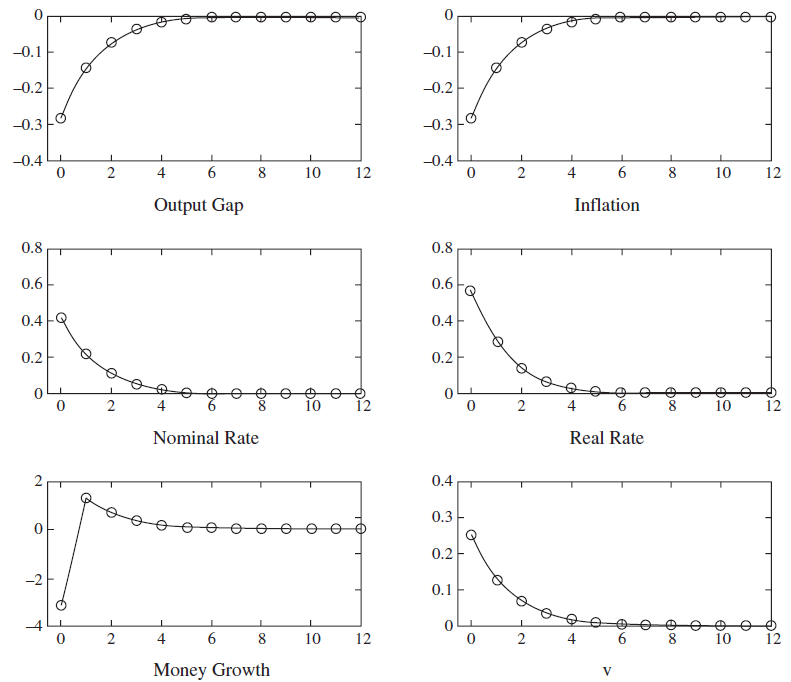
\includegraphics[width=0.75\textwidth]{FIGURES/11_Gali_Fig3_1}
	%\subfigure{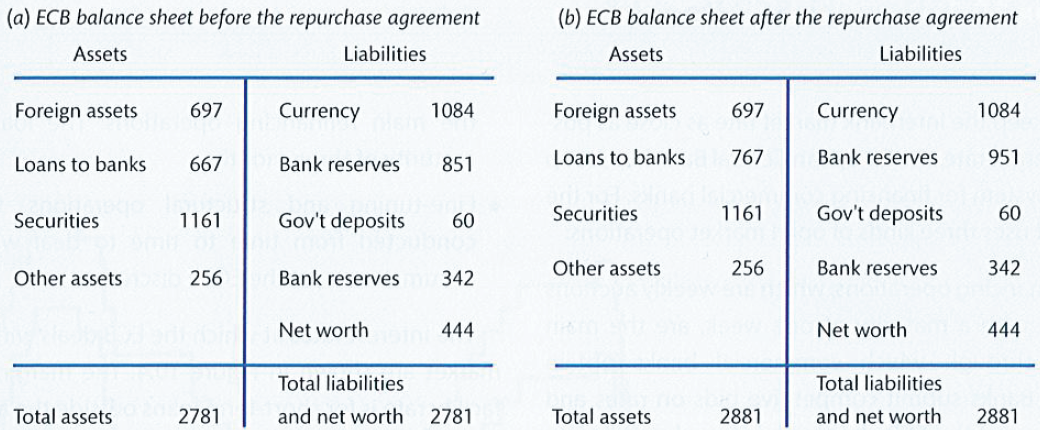
\includegraphics[trim=0 00 0 00,clip,width=0.6\textwidth]{FIGURES/5_CB_balance_sheet_OMO}
	%} 	
	%[trim=left bottom right top
\end{figure}
\vspace{-0.2cm}
\begin{minipage}{0.5\columnwidth}
\tiny
	
\textbf{Source.} Gal\'{i} (2008), Figure 3.1.\\
\end{minipage}
\end{center}

\end{frame}
\end{document}


